\documentclass[10pt]{beamer}

\usetheme{metropolis}
\usepackage{appendixnumberbeamer}

\usepackage{booktabs}
\usepackage[scale=2]{ccicons}

\usepackage{pgfplots}
\usepgfplotslibrary{dateplot}

\usepackage{xspace}

\usefonttheme[onlymath]{serif}

% For PGM
\usepackage{tikz}
\usetikzlibrary{bayesnet}
%\usetikzlibrary{fit,positioning}

\title{Estimating Census Block-Level Citizen Voting Age Population for Redistricting}
\date{\today}
\author{Christopher Wolfram}
%\institute{University of Chicago}

\begin{document}

\maketitle

%\begin{frame}{Table of contents}
%  \setbeamertemplate{section in toc}[sections numbered]
%  \tableofcontents[hideallsubsections]
%\end{frame}

\section{Background}

\begin{frame}{Challenges}
	1. Citizenship data is only available on tracts, but we need it on blocks.
	
	2. The race/ethnicity categories for which we have citizenship data are different from those relevant for litigation.
\end{frame}

\begin{frame}{Redistricting Geography}
	\begin{figure}
		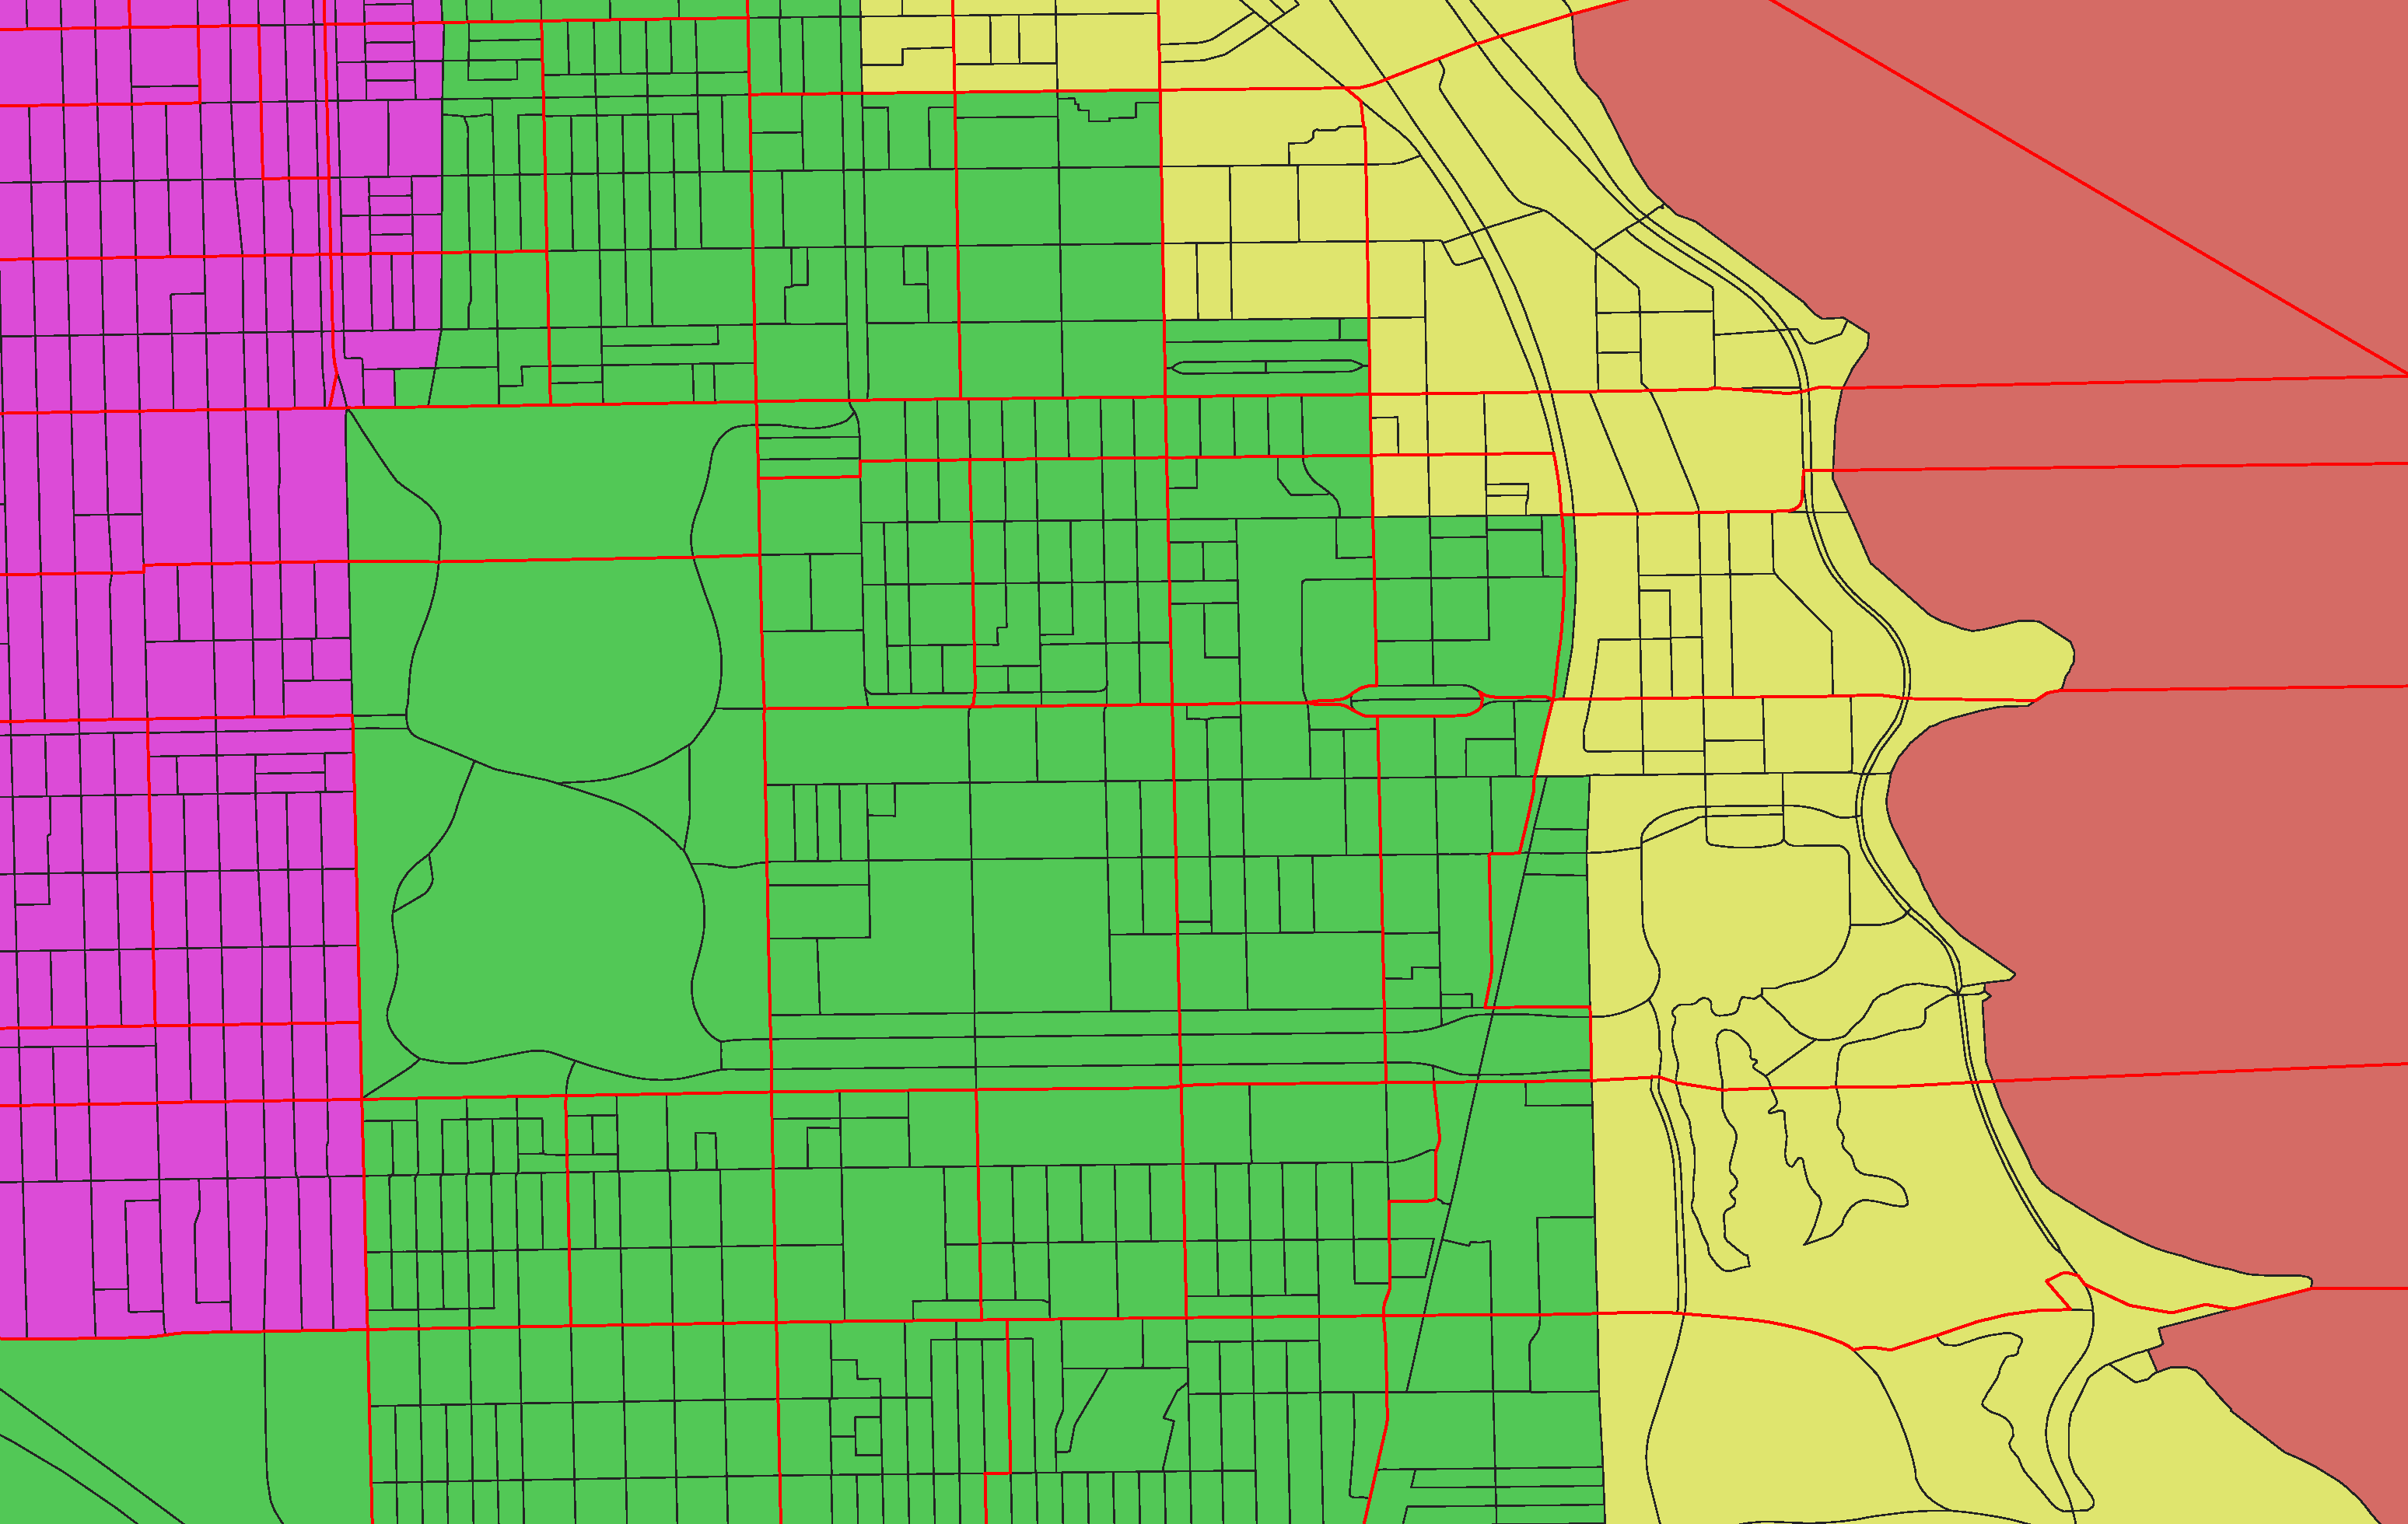
\includegraphics[width=\linewidth]{figures/blockTractMap}
	\end{figure}
\end{frame}

\begin{frame}{Data Sources}
	\begin{itemize}
		\item Decennial Census
		\begin{itemize}
			\item Block-level data
			\item Only gives voting age population (VAP)
			\item Full race/ethnicity breakdown
		\end{itemize}
		\item American Community Survey (ACS)
		\begin{itemize}
			\item Tract level data
			\item Both VAP and CVAP
			\item Only aggregates of race/ethnicity tensor
		\end{itemize}
	\end{itemize}
\end{frame}

\section{From Tracts to Blocks}

\begin{frame}{Naive Disaggregation}
	Let $b$ be some Census Block, and $t$ be the tract containing $b$.
	
	$$CVAP_b \approx CVAP^{ACS}_{t} \frac{VAP^{dec}_b}{VAP^{dec}_t}$$
	
	Or worse, where $A_i$ gives the land area of the geography $i$:
	
	$$CVAP_b \approx CVAP^{ACS}_{t} \frac{A_b}{A_t}$$
\end{frame}

\begin{frame}{ACS vs. Decennial Census}
	\begin{figure}
		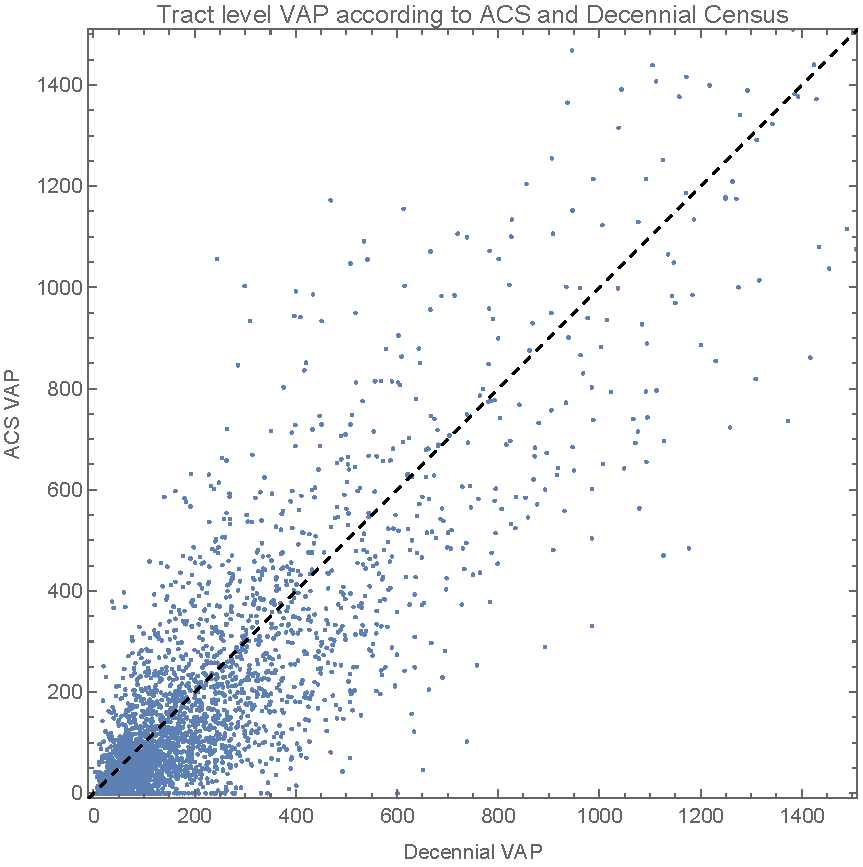
\includegraphics[width=0.6\linewidth]{figures/acsVsDec}
	\end{figure}
\end{frame}

\begin{frame}{Discounted VAP}
	Let $b$ be some Census Block, and $t$ be the tract containing $b$.
	
	$$CVAP_b \approx VAP^{dec}_b\frac{CVAP^{ACS}_{t}}{VAP^{ACS}_{t}}$$
\end{frame}

\begin{frame}{Discounted VAP}
	$$CVAP_b \approx VAP^{dec}_b\frac{CVAP^{ACS}_{t}}{VAP^{ACS}_{t}}$$
	
	\begin{figure}
		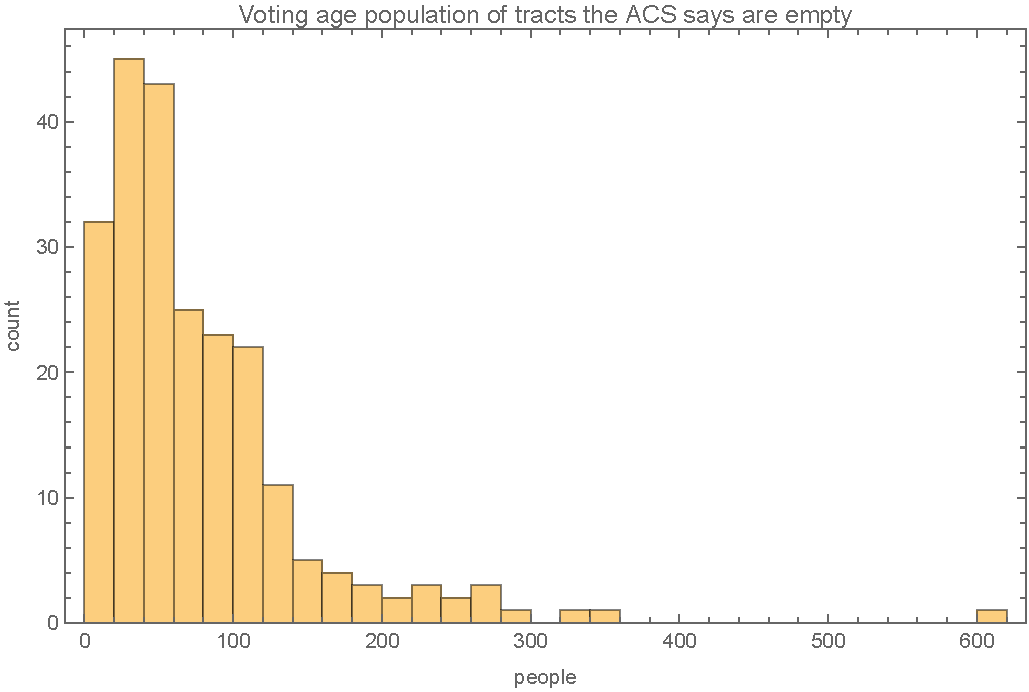
\includegraphics[width=0.7\linewidth]{figures/emptyTracts}
	\end{figure}
\end{frame}

\begin{frame}{Beta-Binomial Model}
For all tracts $t$ and blocks $b$ in $t$,
\begin{align*}
		C_t &\sim \text{Beta}(\alpha,\beta) \\
		CVAP^{ACS}_t &\sim \text{Binomial}(VAP^{ACS}_t, C_t) \\
		CVAP_{t,b} &\sim \text{Binomial}(VAP^{dec}_b, C_t)
\end{align*}
\begin{figure}
\centering
\tikz{
	\node[const](a){$\alpha$};
	\node[const, below=of a](b){$\beta$};
	\node[latent, right=of b](ct){$C_t$};
	\node[obs, right=of ct](cvapt){$CVAP^{ACS}_t$};
	\node[latent, above=of cvapt](cvapb){$CVAP_{t,b}$};
	
	\plate[]{blocks}{(cvapb)}{$b$}
	\plate[]{tracts}{(ct) (cvapt) (cvapb) (blocks)}{$t$}
	
	\edge{a}{ct};
	\edge{b}{ct};
	\edge{ct}{cvapt};
	\edge{ct}{cvapb};
}
\end{figure}
\end{frame}

\begin{frame}{Beta-Binomial Model}
For all tracts $t$ and blocks $b$ in $t$,
\begin{align*}
		C_t &\sim \text{Beta}(\alpha,\beta) \\
		CVAP^{ACS}_t &\sim \text{Binomial}(VAP^{ACS}_t, C_t) \\
		CVAP_{t,b} &\sim \text{Binomial}(VAP^{dec}_b, C_t)
\end{align*}

Posterior:
\begin{align*}
	C_t \mid - &\sim \text{Beta}(\alpha + CVAP^{ACS}_t, \beta +VAP^{ACS}_t - CVAP^{ACS}_t) \\
	CVAP_{t,b} \mid - &\sim \text{BetaBin}(VAP^{dec}_b, \alpha + CVAP^{ACS}_t, \beta +VAP^{ACS}_t - CVAP^{ACS}_t)
\end{align*}

\end{frame}

%\begin{frame}{Beta-Binomial Model}
%\begin{figure}
%\centering
%\begin{tikzpicture}
%\tikzstyle{main}=[circle, minimum size = 10mm, thick, draw =black!80, node distance = 16mm]
%\tikzstyle{connect}=[-latex, thick]
%\tikzstyle{box}=[rectangle, draw=black!100]
%	\node[main, fill = white!100](x)[label=above:$x$]{};
%	\node[main, fill = white!100](y)[below=of x, label=above:$y$]{};
%	\node[main, fill = white!100](ct)[right=of y, label=above:$C_t$]{};
%	\node[main, fill = black!30](cvapt)[right=of ct, label=above:$CVAP^{ACS}_t$]{};
%	\node[main, fill = white!100](cvapb)[right=of cvapt, label=above:$CVAP_b$]{};
%	
%	\path (x) edge [connect] (ct)
%		  (y) edge [connect] (ct)
%		  (ct) edge [connect] (cvapt)
%		  (cvapt) edge [connect] (cvapb);
%	
%	\node[rectangle, inner sep=6.4mm,draw=black!100, fit= (cvapb)]{};
%	\node[rectangle, inner sep=0mm, fit= (cvapb),label=below right:$b$, xshift=2mm, yshift=-1mm]{};
%	
%	\node[rectangle, inner sep=11.4mm,draw=black!100, fit= (ct) (cvapt) (cvapb)]{};
%	\node[rectangle, inner sep=0mm, fit= (ct) (cvapt) (cvapb),label=below right:$t$, xshift=33.5mm, yshift=-6mm]{};
%\end{tikzpicture}
%\end{figure}
%\end{frame}

\begin{frame}{Block-Level Estimates}
	\begin{align*}
&\text{BetaBinomial}(2,82.9532,8.31037) \\
&\text{BetaBinomial}(1,114.953,0.310371) \\
&\text{BetaBinomial}(3,137.953,344.31) \\
&\text{BetaBinomial}(68,193.953,0.310371) \\
&\text{BetaBinomial}(1,205.953,705.31) \\
&\text{BetaBinomial}(12,98.9532,0.310371) \\
&\text{BetaBinomial}(1,88.9532,23.3104) \\
&\text{BetaBinomial}(3,24.9532,11.3104) \\
&\text{BetaBinomial}(4,191.953,193.31) \\
&\text{BetaBinomial}(1,283.953,90.3104) \\
&\text{BetaBinomial}(1,60.9532,18.3104) \\
&\text{BetaBinomial}(6,46.9532,16.3104)
	\end{align*}
	% $$_2F_1(-n,\alpha; \alpha+\beta; 1 - e^{it})$$
\end{frame}

\begin{frame}{Block-Level Estimates}
	\begin{figure}
		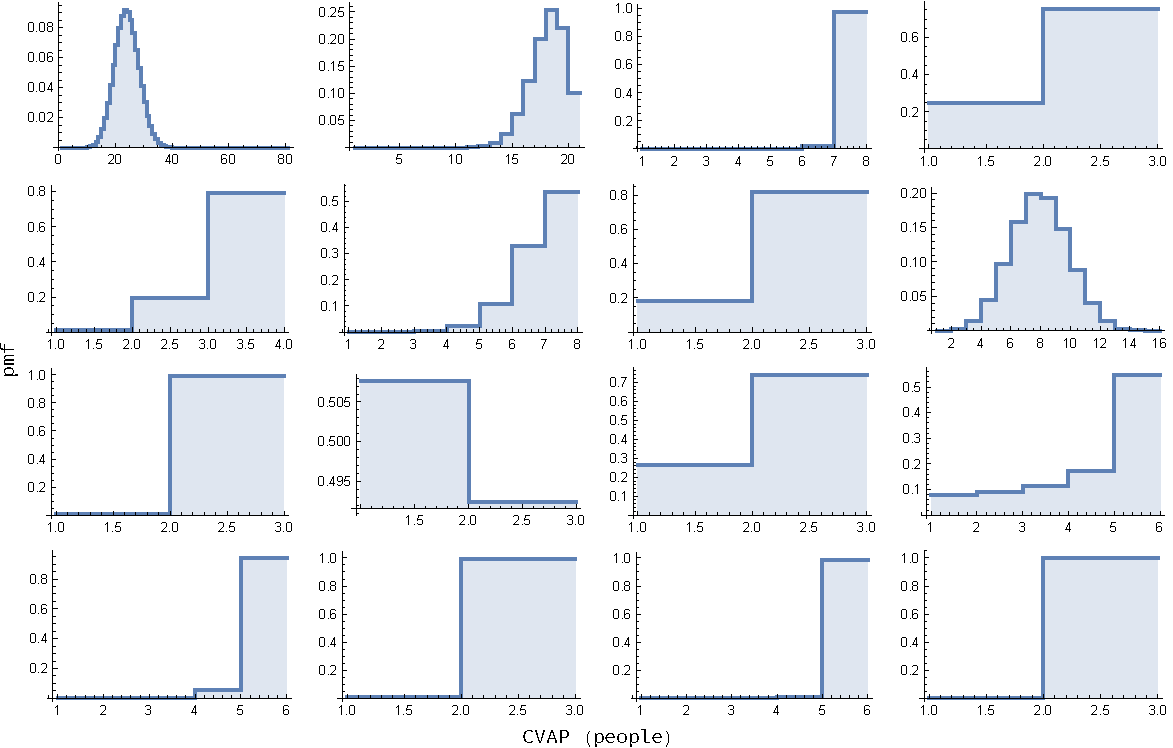
\includegraphics[width=1\linewidth]{figures/blockPMFs}	
	\end{figure}
\end{frame}

\begin{frame}{District-Level Estimates}
	Let $d$ be a congressional district, $b_1, b_2, \dots, b_n$ be the blocks in that district, $p \ast q$ be the convolution of $p$ and $q$, and $\mathcal{F}$ be the Fourier transform.
	
	$$CVAP_d = p_{b_1} \ast p_{b_2} \ast \dots \ast p_{b_n} = \mathcal{F}^{-1}(\mathcal{F}(p_{b_1}) \cdot \mathcal{F}(p_{b_2}) \dots \mathcal{F}(p_{b_n}))$$
\end{frame}

\begin{frame}{District-Level Estimates}
	\begin{figure}
		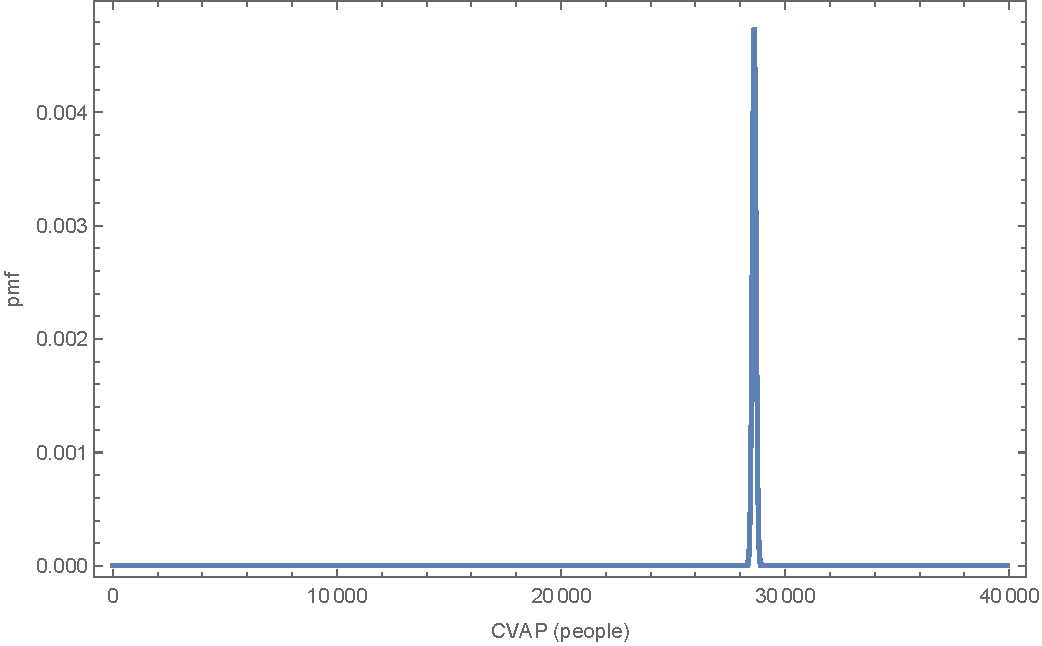
\includegraphics[width=0.6\linewidth]{figures/districtPMFLarge}	
		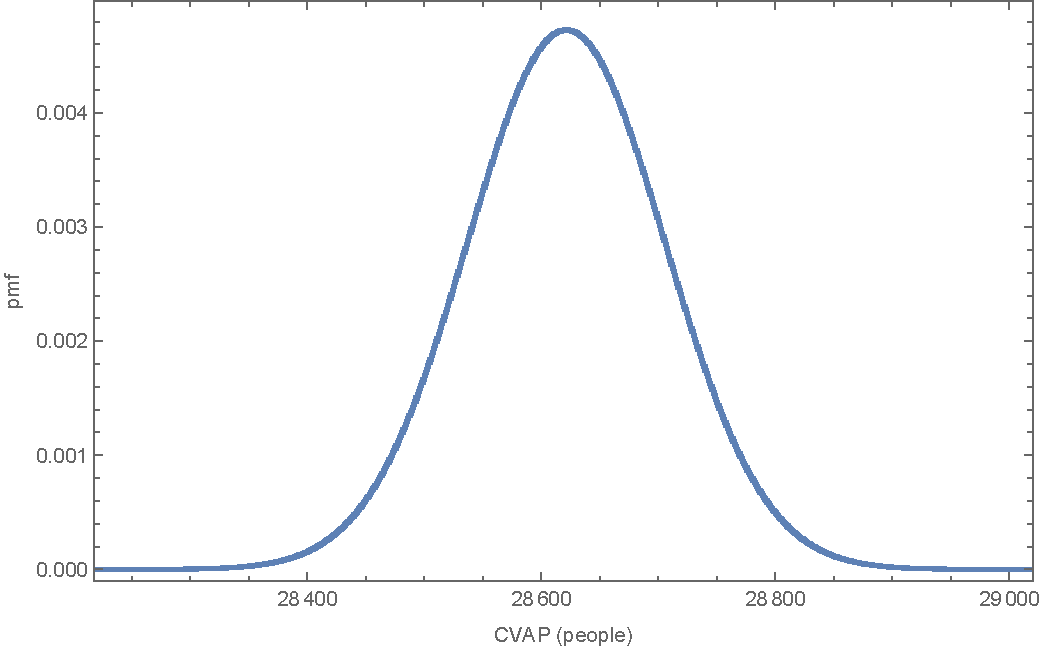
\includegraphics[width=0.6\linewidth]{figures/districtPMFSmall}	
	\end{figure}
\end{frame}

\section{Race/Ethnicity Categories}

\begin{frame}{Race/Ethnicity in the Census}
	\begin{figure}
		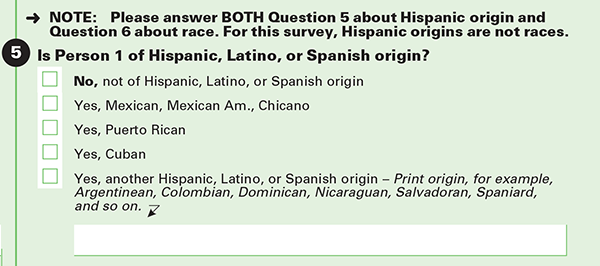
\includegraphics[width=0.6\linewidth]{figures/ethQ}	
		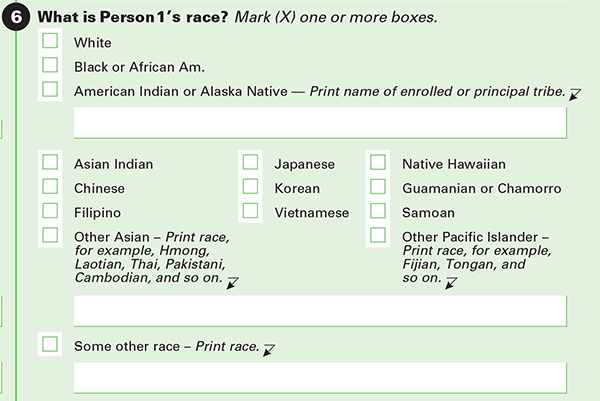
\includegraphics[width=0.6\linewidth]{figures/raceQ}	
	\end{figure}
\end{frame}

\begin{frame}{Race/Ethnicity in the Census}
	ACS race/ethnicity categories:
	\begin{itemize}
		\item White alone
		\item Black or African American Alone
		\item American Indian and Alaska Native Alone
		\item Asian Alone
		\item Native Hawaiian and Other Pacific Islander Alone
		\item Some Other Race Alone
		\item Two or More Races
		\item White Alone, Not Hispanic or Latino
		\item Hispanic or Latino
	\end{itemize}
\end{frame}

\begin{frame}{Litigation Race/Ethnicity Categories}
Per Moon Duchin, the race/ethnicity categories relevant for litigation are:
\begin{itemize}
	\item Any part African American or Black (including part Hispanic)
	\item Hispanic or Latino, but not Black
	\item Any part Asian or Pacific Islander, but not in any above category
	\item Any part Native American, but not in any above category
	\item Any part some other race, but not in any above category
	\item Any part white, but not in any above category
\end{itemize}
\end{frame}

\begin{frame}{Venn Diagram}
	Any part African American or Black (including part Hispanic)
	\begin{figure}
		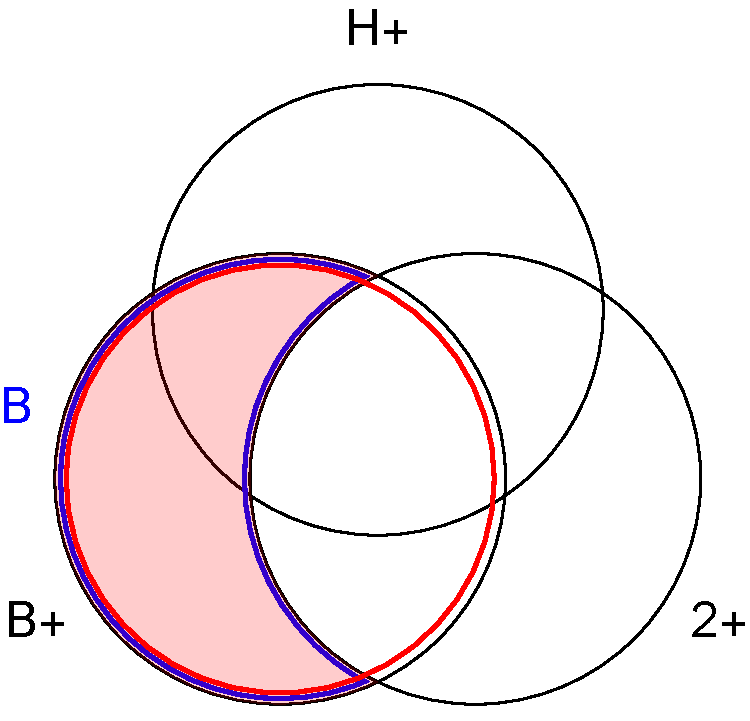
\includegraphics[width=0.5\linewidth]{figures/vennDiagram1}	
	\end{figure}
	$$N(\text{B+}) \approx \underbrace{N(\text{B})}_\text{ACS}+\underbrace{N(\text{2+})}_\text{ACS} \underbrace{p(\text{B+}\mid\text{2+})}_\text{Decennial} = N(\text{B}) + N(\text{2+}) \frac{p(\text{B+}, \text{2+})}{p(\text{2+})}$$
\end{frame}

\begin{frame}{Venn Diagram}
	Hispanic or Latino, but not Black
	\begin{figure}
		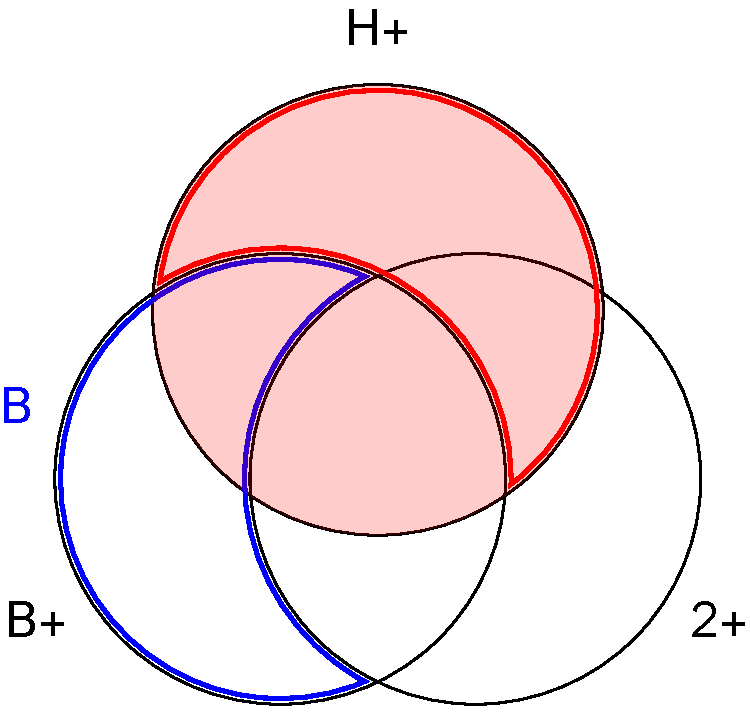
\includegraphics[width=0.5\linewidth]{figures/vennDiagram2}	
	\end{figure}
	$$N(\text{H+})-N(\text{H+})p(\text{B+}\mid\text{H+})$$
\end{frame}

\begin{frame}{Venn Diagram}
	Any part $X$, but not in any above category
	\begin{figure}
		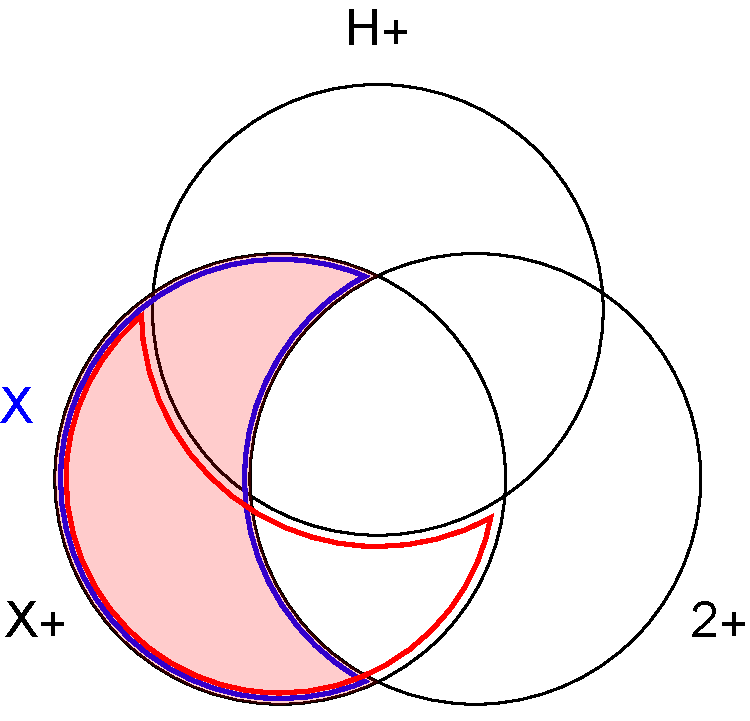
\includegraphics[width=0.5\linewidth]{figures/vennDiagram3}	
	\end{figure}
	$$N(\text{X}) - N(\text{X})p(\text{H+} \mid \text{X}) + N(\text{2+})p(\text{T} \mid \text{2+})$$
	$$N(\text{X}) - N(\text{H+})p(\text{X} \mid \text{H+}) + N(\text{2+})p(\text{T} \mid \text{2+})$$
\end{frame}


\begin{frame}[standout]
 Questions?
\end{frame}

\end{document}
